\documentclass{standalone}
\usepackage{tikz}
\begin{document}


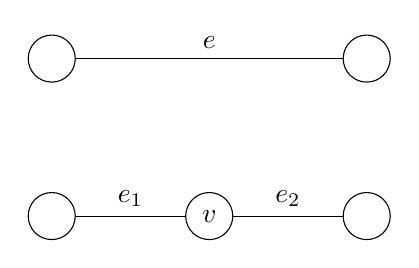
\begin{tikzpicture}
\tikzstyle{vertex}=[circle, draw, minimum size=17pt, inner sep=0pt]
\node[vertex] (A) at (0,0) {};
\node[vertex] (B) at (4,0) {};
\node[vertex] (v) at (2,0) {$v$};

\path 
(v) edge node[above] {$e_1$} (A)
    edge node[above] {$e_2$} (B);

\begin{scope}[yshift=2cm]
\node[vertex] (C) at (0,0) {};
\node[vertex] (D) at (4,0) {};

\path
(C) edge node[above] {$e$} (D);
\end{scope}


\end{tikzpicture}

\end{document}
